\chapter{Implementation}

\section{Simulation application}

Simulation was implemented as a Java application using JDK 1.6. 

\section{Memories}

Each memory implementation implements following IMemory interface:

\begin{lstlisting}[language=Pascal]
interface IMemory {
	Learn(integer foodKind, Point[] locations);
	Point[] GetSample(integer foodkind);	
	(Point, integer) GetExpectedGauss(int foodkind);
}
\end{lstlisting}  

Through the \emph{Learn method} the memory gets new inputs and thus it learns. \emph{GetSample method} returns a sample of food locations according to the agent's believes, it means that based on the information in memory it tries to generate several samples. \emph{GetExpectedGauss method} returns expected Gaussian distribution (x,y location and variance) for the food kind given as a parameter.    

The expected Gaussian distribution is not calculated every time the \emph{GetExpectedGauss method} is called, but it precalculated after the new inputs are processed.

\section{Growing neural gas as a memory}

\begin{figure}      
\begin{center}
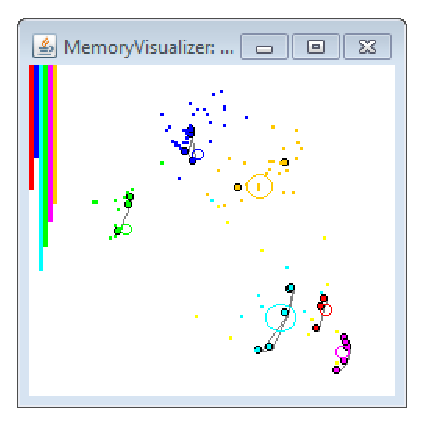
\includegraphics{images/app/gng_screenshot.eps}    
\caption{A visualization of an GNG agent's memory and the situation in the environment. Connected coloured circles represent growing neural gas for each food kind.}
\end{center}                          
\label{app:gngscreenshot}
\end{figure}

Growing neural gas has been explained previously in \ref{usedalgo:gng}. In this section I will explain how that algorithm was used to learn positions of food sources. For this purpose the GNG uses five nodes.

For each kind of food there is a separate GNG engine which learns the believed location of such food. 

\begin{lstlisting}[language=Pascal]
procedure Learn(integer foodkind, Points[] locations)
  gngEngine <- GetEngineByFoodKind(foodkind)
  gngEngine.SetDescreteSignals(locations)
end
\end{lstlisting}  

\emph{SetDescreteSignals method} assigns known food locations (array of x,y points) to the neural network so as to be later processed using the GNG algorithm described in \ref{usedalgo:gng}. At the end of day, i.e. end of each simulation step, the learnt information is processed by the GNG.

When the memory is asked about expected Gauss distribution, it uses the five nodes in the GNG to compute it.

\section{Grid as a memory}

\begin{figure}      
\begin{center}
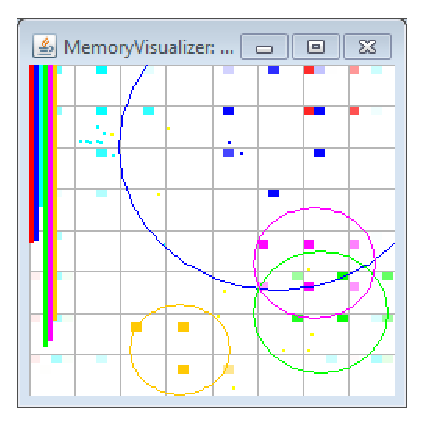
\includegraphics{images/app/grid_screenshot.eps}    
\caption{A visualization of an grid agent's memory and the situation in the environment. The coloured bars on the left side show current levels of agent's hunger. Coloured squares display grid cell values.}
\end{center}                          
\label{app:gridscreenshot}
\end{figure}

As in GNG memory implementation, the grid memory uses \emph{Learn method} to update current state. 

\begin{lstlisting}[language=Pascal]
procedure Learn(integer foodkind, Points[] locations)
   grid <- GetGridByFoodKind(foodkind)
   hasInput <- CreateEmptyMatrix(cols, rows)
   
   for (x, y) in locations do
   begin
      (gridX, gridY) <- GetGridCoords(x, y)
      grid[gridX, gridY]++;
   end 
   
   for (i, j) in grid do
   begin
      cell <- grid[i, j]
      if hasInput[i, j] > 0 then
        cell.IncPositive()
      else
        if node is in sight distance then
          cell.IncNegative()
   end
end
\end{lstlisting}  

An actuall value of the cell is computed using following formula:

\begin{equation}        
\begin{split}
value = positive - negative / \alpha  \\
if (value < 0) value = 0 
\end{split}
\end{equation}  

$\alpha$ is set to 2.

The gaussian distribution is computed following way:

\begin{itemize}
\item x, y position is computed as a weighted mean of cells: 
\begin{equation}
  \frac{\sum{CellValue_i\times (x_i,y_i)}}{\sum{CellValue_i}}
\end{equation}
\item variance is computed as normalized sum of weighted distances:
\begin{equation}
\frac{\sum{DistanceToCenter_i\times CellValue_i}}{\alpha\times NumPositiveCells\times MaxCellValue}
\end{equation}
\end{itemize}








                                    